\documentclass{article}
\usepackage{hyperref}
\usepackage{graphicx}
\usepackage{subfigure}
\usepackage{listing}
\usepackage[export]{adjustbox}
\usepackage{xepersian}
\settextfont{Vazirmatn.ttf}
\hypersetup{colorlinks,linkcolor={black},citecolor={black},urlcolor={black}}
\begin{document}
\begin{titlepage}
    \centering
    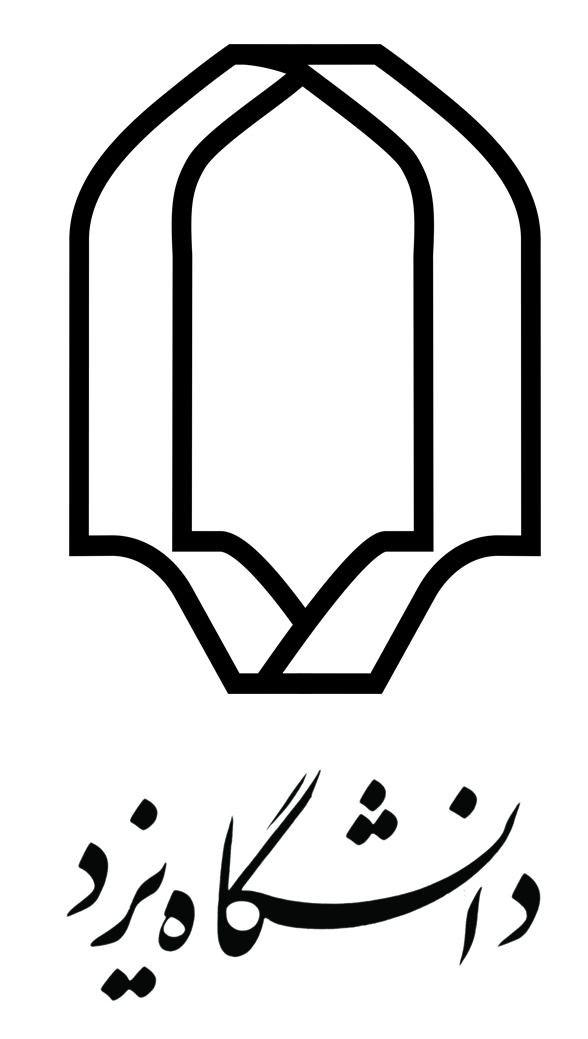
\includegraphics[width=0.2\textwidth]{logoYazdUniversity.png}\\[1cm] 
    \textsc{\Large \bfseries الگوریتم درخت کارتزینی}\\[0.5cm] 
    \textbf{شروین خیرخواه}\\[0.5cm] 
    \textbf{خرداد ۱۴۰۳}\\[0.5cm]
\end{titlepage}
\tableofcontents
\newpage
\section{مقدمه و تاریخچه ایجاد الگوریتم}
اولین بار الگوریتم درخت کارتزینی توسط "ژان وویمین" (  Vuillemin Jean ) در سال 1980 در زمینه ساختارهای داده جستجوی کران ( structure data search range ) معرفی شد.

هدف اولیه از معرفی این الگوریتم، ایجاد ساختاری کارآمد برای یافتن حداقل یا حداکثر مقدار در یک بازه از آرایه بود.

درخت‌های کارتزینی به دلیل سادگی، کارایی و قابلیت تعمیم به سرعت محبوبیت پیدا کردند و در زمینه‌های مختلف علوم کامپیوتر از جمله جستجوی دودویی، حل مسائل مربوط به بازه‌ها و ساختارهای داده تَرَپ ( Treap ) مورد استفاده قرار گرفتند.

\begin{center}
    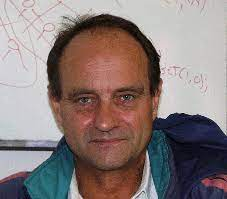
\includegraphics[scale=0.7]{firsti.jpg}
\end{center}
\begin{center}
    \small ژان وویمین
\end{center}
\section{علت ایجاد الگوریتم}
در آن زمان، ساختارهای داده مختلفی برای ذخیره و جستجوی اطلاعات وجود داشت. برخی از این ساختارها مانند آرایه‌ها و لیست‌های پیوسته، برای جستجوی عناصر به صورت تصادفی کارآمد بودند، اما برای یافتن حداقل یا حداکثر مقدار در یک بازه از آرایه، کارایی لازم را نداشتند.

ساختارهای داده دیگری مانند درخت‌های دودویی جستجو، برای یافتن حداقل یا حداکثر مقدار در یک بازه کارآمدتر بودند، اما درج و حذف عناصر در آن‌ها می‌توانست عملیات پرهزینه‌ای باشد.

الگوریتم درخت کارتزینی با ارائه روشی برای ساخت یک درخت دودویی متعادل از یک آرایه، این چالش‌ها را حل کرد. این درخت‌های متعادل، عملیات جستجو، درج و حذف را در زمان ( n log ) انجام می‌دهند، که در مقایسه با سایر ساختارهای داده موجود در آن زمان، بسیار کارآمدتر بود.

علاوه بر کارایی، درخت‌های کارتزینی به دلیل سادگی و قابلیت تعمیم نیز مورد توجه قرار گرفتند. پیاده‌سازی این الگوریتم نسبتاً ساده است و می‌توان از آن برای حل طیف وسیعی از مسائل مربوط به جستجو و پردازش بازه‌ها استفاده کرد.

\section{توضیح الگوریتم}
\subsection{درخت در علوم کامپیوتر}
در علوم کامپیوتر، درخت (Tree) یک ساختار داده سلسله مراتبی است که از گره‌ها (Nodes) و یال‌ها (Edges) تشکیل شده است. در این ساختار، هر گره می‌تواند به صفر یا تعداد بیشتری گره دیگر به عنوان فرزند (Child) متصل باشد.

درخت‌ها به دلیل ساختار سازمان‌یافته و قابلیت پیمایش کارآمد، در زمینه‌های مختلف علوم کامپیوتر کاربردهای فراوانی دارند.
\newline ویژگی‌های کلیدی درخت:
\newline ریشه: گره‌ای که در بالاترین سطح درخت قرار دارد و هیچ فرزندی ندارد.
\newline فرزندان: گره‌هایی که به طور مستقیم به یک گره دیگر متصل هستند.
\newline سطح: فاصله گره از ریشه. ریشه در سطح ( 0 ) قرار دارد.
\newline زیر درخت: شامل ریشه و تمام فرزندان و نوادگان آن.
\newline برگ: گره‌ای که هیچ فرزندی ندارد.
\newline درجه: تعداد فرزندان یک گره.

\subsection{درخت دودویی}
درخت دودویی ( tree binary ) یک ساختار داده بنیادی در علم کامپیوتر است. این ساختار سلسله مراتبی شبیه به یک درخت با یک گره خاص به نام ریشه (Root) است. گره‌های موجود در یک درخت دودویی می‌توانند حداکثر دو فرزند داشته باشند: یک فرزند چپ و یک فرزند راست. این فرزندان خود می‌توانند درخت‌های دودویی باشند و یک ساختار بازگشتی (Recursive) ایجاد کنند.
\newline ویژگی‌های کلیدی یک درخت دودویی :
\newline گره ریشه: نقطه شروع درخت است. هر درخت دودویی دقیقاً یک گره ریشه دارد.
\newline فرزندان: هر گره به جز برگ‌ها (که در ادامه توضیح داده می‌شود)، می‌تواند تا دو فرزند داشته باشد: فرزند چپ و فرزند راست.
\newline گره‌های برگ: گره‌هایی که هیچ فرزندی ندارند، برگ نامیده می‌شوند. 
\newline ساختار بازگشتی: یک درخت دودویی را می‌توان به زیر درخت‌های (Sub-Tree) کوچکتری تقسیم کرد. این زیر درخت‌ها خود می‌توانند درخت‌های دودویی باشند که یک ساختار سلسله مراتبی را ایجاد می‌کنند.
\subsection{توده (Heap) }
توده (Heap) یک ساختار داده درختی مبتنی بر آرایه است که از خاصیت توده پیروی می‌کند. در توده ماکس، مقدار هر گره بزرگتر یا مساوی با مقادیر هر دو فرزندش است. در مقابل، در توده مین، مقدار هر گره کوچکتر یا مساوی با مقادیر هر دو فرزندش است.
\newline الگوریتم ساخت توده :
\newline ایجاد توده اولیه: آرایه ورودی را به عنوان یک درخت دودویی کامل در نظر بگیرید. هر عنصر در آرایه به عنوان یک گره در درخت عمل می‌کند.
\newline نظیم توده: از پایین‌ترین سطح درخت به سمت بالا حرکت کنید. برای هر گره، مقادیر آن و دو فرزندش را مقایسه کنید.
\newline  اگر مقدار گره کوچکتر از یکی از فرزندانش باشد، جای آن را با فرزند بزرگتر عوض کنید. این کار را به طور مکرر برای هر گره تا زمانی که به ریشه برسید، انجام دهید.

\begin{center}
   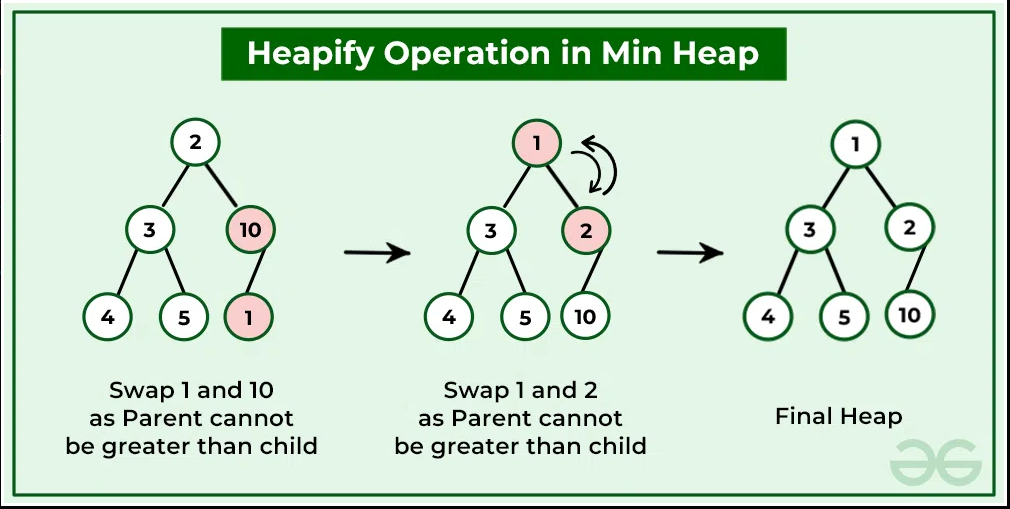
\includegraphics[scale=0.3]{heap.png}
\end{center}
\begin{center}
    \small الگوریتم هیپ کردن
\end{center}
\subsection{درخت کارتزینی چیست؟}
درخت کارتزینی ( tree cartesian ) یک ساختار داده است که بر روی یک آرایه از اعداد تعریف می‌شود. در این ساختار، هر عضو آرایه به یک گره در درخت تبدیل می‌شود. ویژگی منحصر به فرد درخت کارتزینی این است که اگر پیمایش آن به صورت درون‌تراز ( In-Order ) انجام شود، ترتیب عناصر در خروجی دقیقاً با ترتیب عناصر در آرایه اصلی مطابقت دارد.

علاوه بر این، درخت کارتزینی خاصیت هرم کمینه ( Min Heap ) را نیز دارا است. به این معنی که در هر زیر درخت، کلید ریشه کوچک‌تر از کلید تمام گره‌های فرزند آن است.
\section{نحوه ساخت درخت کارتزینی}
برای ساخت درخت کارتزینی از یک آرایه، مراحل زیر را دنبال می‌کنیم:

\newline مقادیر کمینه را پیدا کنید: ابتدا، کمینه کل آرایه را پیدا می‌کنیم. این مقدار به عنوان ریشه درخت کارتزینی در نظر گرفته می‌شود.
\newline درخت‌های فرعی را بسازید: سپس به طور بازگشتی، دو درخت فرعی برای ریشه ایجاد می‌کنیم. درخت فرعی سمت چپ شامل تمام عناصری در آرایه است که کوچک‌تر از ریشه هستند. درخت فرعی سمت راست نیز شامل تمام عناصری در آرایه است که بزرگ‌تر از ریشه هستند.
\newline درخت را کامل کنید: در نهایت، درخت فرعی سمت چپ را به عنوان فرزند چپ ریشه و درخت فرعی سمت راست را به عنوان فرزند راست ریشه قرار می‌دهیم.
\newline با استفاده از این الگوریتم بازگشتی، می‌توان درخت کارتزینی را برای یک آرایه از n عنصر ساخت.
\begin{center}
    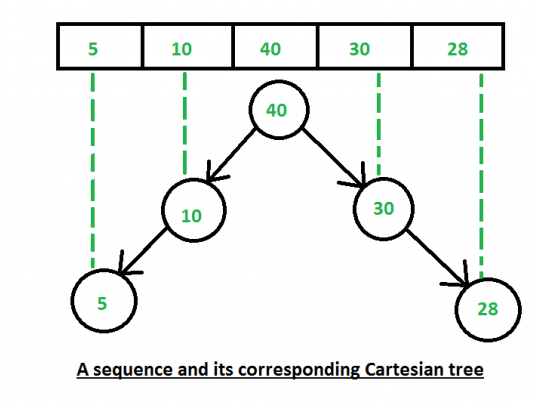
\includegraphics[scale=0.3]{second.png}
\end{center}
\begin{center}
    \small هیپ ماکسیمم
\end{center}
\begin{center}
    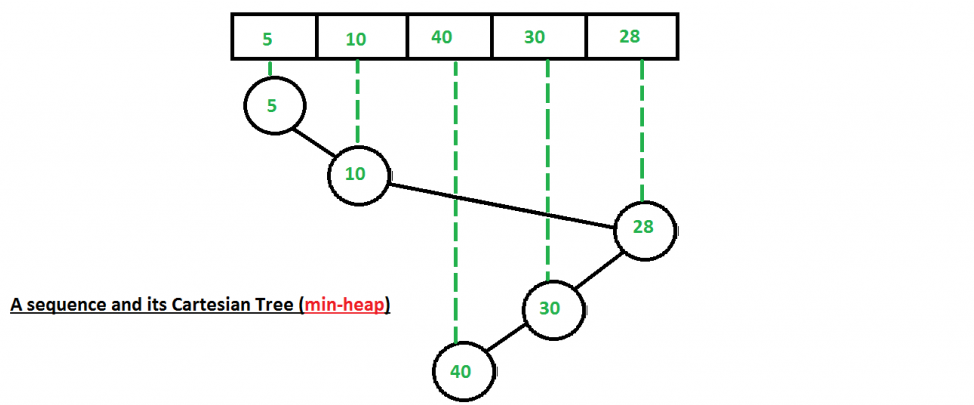
\includegraphics[scale=0.3]{third.png}
\end{center}
\begin{center}
    \small هیپ مینیمم
\end{center}
\section{بررسی الگوریتم و فلوچارت}
\subsection{عملکرد}
\newline این الگوریتم با استفاده از تکنیک بازگشتی ( Recursion ) به صورت زیر عمل می‌کند:
\newline مقادیر کمینه را پیدا کنید: ابتدا، کمینه ( min ) را در آرایه پیدا می‌کنیم.
\newline یک گره جدید با مقدار min به عنوان ریشه درخت کارتزینی ایجاد می‌کنیم.
\newline زیرآرایه سمت چپ ( leftSubarray ): از عناصر آرایه اصلی که کوچک‌تر از min هستند، یک زیرآرایه جدید ایجاد می‌کنیم.
\newline زیرآرایه سمت راست ( rightSubarray ): از عناصر آرایه اصلی که بزرگ‌تر از min هستند، یک زیرآرایه جدید ایجاد می‌کنیم.
\newline به طور بازگشتی: برای هر زیرآرایه ( leftSubarray ) و ( rightSubarray ) مراحل 1 تا 3 را تکرار می‌کنیم تا زمانی که تمام عناصر آرایه اصلی در درخت کارتزینی قرار بگیرند.
\newline درخت را کامل کنید: در نهایت، گره ریشه ( min ) را به عنوان ریشه درخت کارتزینی نهایی در نظر می‌گیریم و فرزندان آن را به ترتیب درخت‌های فرعی ساخته شده از leftSubarray و rightSubarray در مراحل قبل، به آن متصل می‌کنیم.
\subsection{فلوچارت}
\begin{figure}
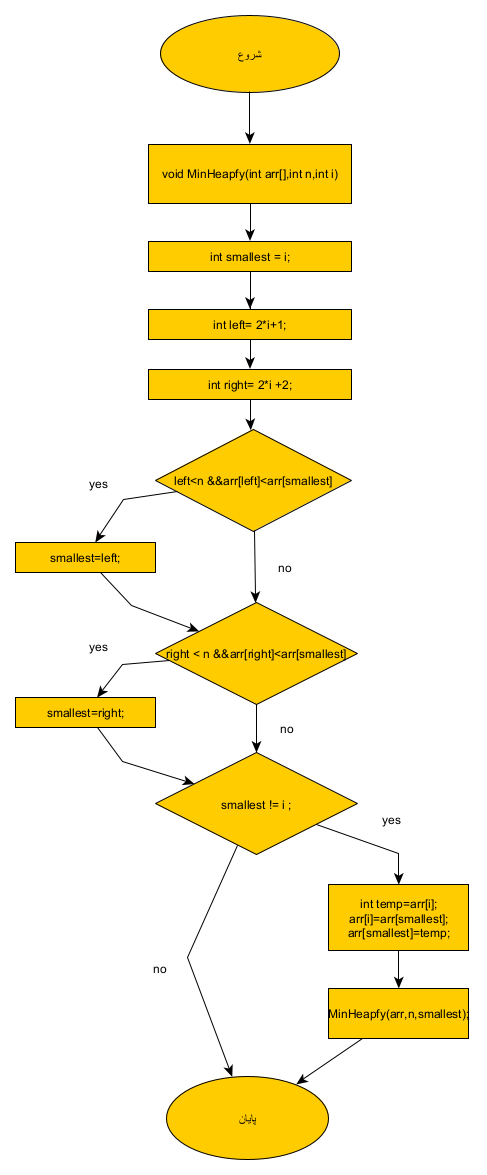
\includegraphics[max size={\textwidth}{\textheight}]{unnamed0.png}
\end{figure}

\begin{figure}
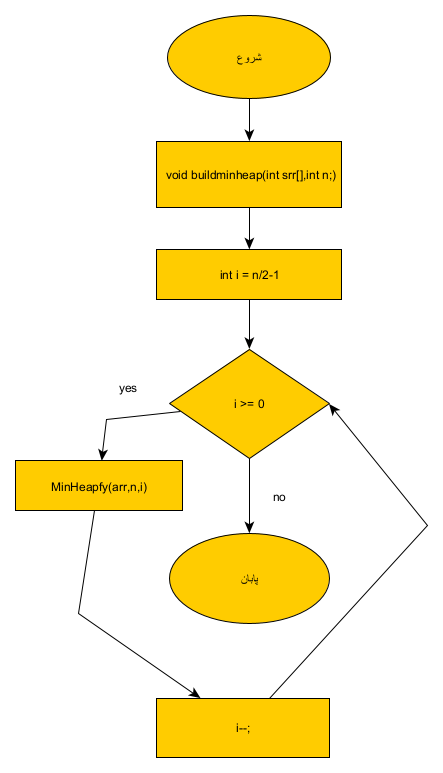
\includegraphics[max size={\textwidth}{\textheight}]{unnamed1.png}
\end{figure}

\subsection{کد}
\begin{latin}
\begin{verbatim}
    import java.util.Scanner;

class CTNode {
    CTNode left, right;
    int value;

    public CTNode() {
        left = null;
        right = null;
        value = 0;
    }
}

class CartesianTree {
    private CTNode root;

    public CartesianTree(int[] data) {
        root = build(data);
    }

    public CTNode build(int[] data) {
        if (data == null || data.length == 0) {
            return null;
        }
        return build(data, 0, data.length - 1);
    }

    private CTNode build(int[] data, int start, int end) {
        if (end < start) {
            return null;
        }
        int min = Integer.MAX_VALUE;
        int minIndex = -1;
        for (int i = start; i <= end; i++) {
            if (data[i] < min) {
                min = data[i];
                minIndex = i;
            }
        }
        CTNode node = new CTNode();
        node.value = min;
        node.left = build(data, start, minIndex - 1);
        node.right = build(data, minIndex + 1, end);
        return node;
    }

    public boolean isEmpty() {
        return root == null;
    }

    public int countNodes() {
        return countNodes(root);
    }

    private int countNodes(CTNode r) {
        if (r == null) {
            return 0;
        } else {
            int l = 1;
            l += countNodes(r.left);
            l += countNodes(r.right);
            return l;
        }
    }

    public void inorder() {
        inorder(root);
    }

    private void inorder(CTNode r) {
        if (r != null) {
            inorder(r.left);
            System.out.print(r.value + " ");
            inorder(r.right);
        }
    }

    public void preorder() {
        preorder(root);
    }

    private void preorder(CTNode r) {
        if (r != null) {
            System.out.print(r.value + " ");
            preorder(r.left);
            preorder(r.right);
        }
    }

    public void postorder() {
        postorder(root);
    }

    private void postorder(CTNode r) {
        if (r != null) {
            postorder(r.left);
            postorder(r.right);
            System.out.print(r.value + " ");
        }
    }
}

public class CartesianTreeTest {
    public static void main(String[] args) {
        Scanner scan = new Scanner(System.in);
        System.out.println("Cartesian Tree Test\n");
        System.out.println("Enter number of integer values");
        int N = scan.nextInt();
        int arr[] = new int[N];
        System.out.println("\nEnter " + N + " integer values");
        for (int i = 0; i < N; i++) {
            arr[i] = scan.nextInt();
        }
        CartesianTree ct = new CartesianTree(arr);
        System.out.println("\nTree Details :");
        System.out.println("Empty status - " + ct.isEmpty());
        System.out.println("No of nodes - " + ct.countNodes());
        System.out.print("Post order : ");
        ct.postorder();
        System.out.print("\nPre order : ");
        ct.preorder();
        System.out.print("\nIn order : ");
        ct.inorder();
        System.out.println();
    }
}  
\end{verbatim}
\end{latin}
\subsection{کلاس ها}
CTNode : این کلاس نشان دهنده یک گره (Node) واحد در درخت کارتزینی است. سه ویژگی دارد:
\begin{itemize}
    \item left : اشاره به گره فرزند چپ.
    \item right : اشاره به گره فرزند راست.
    \item value : مقدار عددی ذخیره شده در گره.
\end{itemize}
CartesianTree : این کلاس کل درخت کارتزی را نشان می دهد. قابلیت های زیر را دارد:
\begin{itemize}
    \item سازنده : یک آرایه اعداد صحیح را به عنوان ورودی می گیرد و از آن درخت کارتزی را می سازد.
    \item build : این تابع به طور بازگشتی درخت کارتزی را از یک آرایه داده شده می سازد. کمترین عنصر آرایه را پیدا می کند و آن را به عنوان ریشه (Root) قرار می دهد. سپس به طور بازگشتی زیر درخت چپ را با عناصر کوچکتر از ریشه و زیر درخت راست را با عناصر بزرگتر از ریشه می سازد.
    \item isEmpty : بررسی می کند که آیا درخت خالی است (گره ریشه ندارد).
    \item countNodes :  تعداد کل گره های درخت را می شمارد.
    \item inorder, preorder, postorder : این توابع به ترتیب پیمایش های درون بر ( Inorder )، پیش بر ( Preorder ) و پس بر ( Postorder ) درخت را انجام می دهند. هر تابع پیمایش یک تابع کمکی با همین نام را برای انجام پیمایش بازگشتی و چاپ مقادیر گره ها فراخوانی می کند.
\end{itemize}
\subsection{کلاس اصلی}
\begin{itemize}
    \item از کاربر می خواهد تعداد مقادیر عددی را که می خواهد در درخت ذخیره کند وارد کند.
    \item مقادیر صحیح را از کاربر می خواند و آنها را در یک آرایه ذخیره می کند.
    \item با ارسال آرایه به سازنده، یک شیء CartesianTree ایجاد می کند.
    \item بررسی می کند که آیا درخت خالی است و نتیجه را چاپ می کند.
    \item تعداد گره های درخت را می شمارد و تعداد را چاپ می کند.
    \item یک پیمایش پس بر از درخت انجام می دهد و مقادیر گره های بازدید شده را چاپ می کند.
    \item یک پیمایش پیش بر از درخت انجام می دهد و مقادیر گره های بازدید شده را چاپ می کند.
    \item یک پیمایش درون بر از درخت انجام می دهد و مقادیر گره های بازدید شده را چاپ می کند.
\end{itemize}
\section{کاربردها}
\subsection{ ساختارهای داده}
درخت‌های جستجوی بهینه: درخت‌های کارتزینی می‌توانند به عنوان ساختار داده‌ای کارآمد برای جستجوی عناصر در یک مجموعه مرتب شده عمل کنند. زمان جستجو در این درختان در بدترین حالت ( n log ) است که با درخت‌های جستجوی دودویی متعادل مانند درخت‌های AVL یا درخت‌های سرخ همسان است.
\subsection{ماشین لرنینگ}
انتخاب ویژگی: درخت‌های کارتزینی می‌توانند برای انتخاب ویژگی‌ها در الگوریتم‌های یادگیری ماشین استفاده شوند. این کار با شناسایی ویژگی‌هایی که اطلاعات بیشتری در مورد هدف ارائه می‌دهند و حذف ویژگی‌های تکراری یا بی‌فایده انجام می‌شود.
\newline طبقه‌بندی: درخت‌های کارتزینی می‌توانند برای طبقه‌بندی داده‌ها به دو دسته یا بیشتر استفاده شوند. این کار با تقسیم داده‌ها بر اساس ویژگی‌های انتخاب شده و تکرار فرآیند در زیرمجموعه‌ها انجام می‌شود.
\newline رگرسیون: درخت‌های کارتزینی می‌توانند برای پیش‌بینی مقادیر پیوسته (رگرسیون) استفاده شوند. این کار با ساختن یک مدل رگرسیونی در هر زیرشاخه از درخت و ترکیب پیش‌بینی‌ها در سطوح بالاتر انجام می‌شود.
\subsection{ پردازش زبان طبیعی}
تجزیه و تحلیل نحوی: درخت‌های کارتزینی می‌توانند برای تجزیه و تحلیل ساختار نحوی جملات زبان طبیعی استفاده شوند. این کار با شناسایی وابستگی‌های بین کلمات و ساختن یک درخت نحوی از جمله انجام می‌شود.
\newline استخراج اطلاعات: درخت‌های کارتزینی می‌توانند برای استخراج اطلاعات از متن، مانند نام افراد، مکان‌ها یا تاریخ‌ها استفاده شوند. این کار با شناسایی الگوهای خاص در متن و مرتبط کردن آنها با اطلاعات مربوطه انجام می‌شود.
\subsection{ گرافیک کامپیوتری}
مدل‌سازی سه‌بعدی: درخت‌های کارتزینی می‌توانند برای مدل‌سازی سه‌بعدی اشیاء و صحنه‌ها استفاده شوند. این کار با ساختن یک سلسله مراتب از گره‌ها انجام می‌شود که هر کدام نشان‌دهنده بخشی از مدل هستند.
\newline رندرینگ: درخت‌های کارتزینی می‌توانند برای رندرینگ گرافیک سه‌بعدی استفاده شوند. این کار با پیمایش درخت و رسم هر گره و فرزندان آن انجام می‌شود.
\section{نتیجه گیری}
در مجموع، درخت‌های کارتزینی به دلیل ساختار ساده و کارآمد خود، ابزاری قدرتمند برای حل طیف وسیعی از مسائل در علوم کامپیوتر، به ویژه یادگیری ماشین، هستند. آنها به طور فزاینده‌ای در تحقیقات و کاربردهای مختلف مورد استفاده قرار می‌گیرند.
\section{منابع}
\begin{latin}
\begin{itemize}
\item GeeksforGeeks - Cartesian Tree
\item Bender, Michael A.; Farach-Colton, Martin (2000), "The LCA problem revisited",
\item Berkman, Omer; Schieber, Baruch; Vishkin, Uzi (1993), "Optimal doubly logarithmic parallel algorithms based on finding all nearest smaller values",
\item ishimoto, Akio; Fujisato, Noriki; Nakashima, Yuto; Inenaga, Shunsuke (2021), "Position heaps for Cartesian-tree matching on strings and tries", in Lecroq,
\item Levcopoulos, Christos; Petersson, Ola (1989), "Heapsort - Adapted for Presorted Files"
\end{itemize}
\end{latin}
\end{document}